\section{Demosaicing}
\label{sec:Demosaicing}
\subsection{Bakgrunn}
En både økonomisk og praktisk måte å fange opp primærfarger på er å plassere et fargefilter over fargesensorene i et kamera. Det finnes ulike filtre, men det mest populære er Bayer-filteret \cite{Demosaic38:online}, illustrert ved Figur \ref{Figur 2}. Ved å se på sensoren som en matrise og legge på ulike fargefiltre på de individuelle elementene kan en samle informasjon ved å la de respektive pikslene fange lysstyrken i sitt område. Denne informasjonen er tilstrekkelig til å gjøre veldig nøyaktige gjett om den ekte fargen i dette området. Nettopp denne metoden som ser på omkringliggende piksler for å estimere verdier, kalles interpolasjon \footnote{\url{https://en.wikipedia.org/w/index.php?title=Interpolation&oldid=949792579}}.
\begin{figure}
\begin{center}
    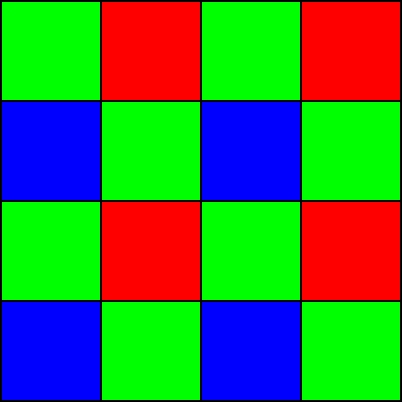
\includegraphics[width=0.3\columnwidth]{bilder/Bayer_pattern.png}
    \caption{Bayer filter \label{Figur 2}} \source{Wikipedia bidragsytere~\cite{wiki:color}}
\end{center}
\end{figure}
Bayer-filteret er et mønster som alternerer mellom en rad av grønne og røde piksler, og en rad av blå og grønne piksler (\ref{Figur 2}). Fra dette ser man enkelt at det finnes dobbelt så mange grønne piksler, som det gjør røde og blå. Dette er fordi fargereseptorene som sitter på netthinnen i menneskeøyet er mer følsomme for grønt lys. På netthinnen finnes omtrent 6 millioner tapper av typene S, L og M-tapper. S-tappene registrerer fiolett, altså blandinger mellom rød og blå \cite{wiki:lilla}. Derimot registrerer både L -og M-tapper grønt, med mest følsomhet rundt bølgelengder tilsvarende 534-564nm \cite{wiki:coneCell}. Dermed trenger en mer informasjon fra grønne piksler for å produsere et bilde som menneskeøyne vil kunne oppfatte som naturtro.

\subsection{Implementasjon}
Fra kamerasensoren kommer en gråtonemosaikk, som i praksis altså er mengden lys i hver av de tre fargekanalene, R, G og B. For implementasjon i Python kan man simulere denne mosaikken ved å betrakte et bilde \texttt{im} representert ved en $M\times N \times 3$ \texttt{numpy array}. Da kan gråtonemosaikken lages slik:
\begin{lstlisting}[language=Python]
mosaic = np.zeros(im.shape[:2])        #Alloker plass
mosaic[ ::2, ::2] = im[ ::2, ::2, 0]   #R 
mosaic[1::2, ::2] = im[1::2, ::2, 1]   #G
mosaic[ ::2, 1::2] = im[ ::2, 1::2, 1] #G
mosaic[1::2, 1::2] = im[1::2, 1::2, 2] #B
\end{lstlisting}
Videre kan en flytte informasjonen fra moisaikken inn i det ønskede fargebildet. Dette gjøres enkelt ved og for hver dimensjon i det nye bildet, fylle inn med informasjon fra hver av dimensjonene R, G og B fra mosaikken. Også her må man ta høyde for at grønne piksler forekommer dobbelt så ofte som de andre \cite{Demosaic38:online}. Videre kan en bruke inpainting beskrevet i (\ref{sec:Inpainting}) for å fylle inn den manglende informasjonen. Dette gjøres ved å definere en maske $\Omega_i$ for hver av fargekanalene. Deretter gjøres et funksjonskall til inpainting-algoritmen for hver dimensjon, der \texttt{im\_ed} er det resulterende fargebildet:
\begin{lstlisting}[language=Python]
eks.Inpainting_mosaic(im_ed[:,:,0], mask[:,:,0])
eks.Inpainting_mosaic(im_ed[:,:,1], mask[:,:,1])
eks.Inpainting_mosaic(im_ed[:,:,2], mask[:,:,2])
\end{lstlisting}
\begin{figure}
\begin{center}
    
\end{center}
\end{figure}

\begin{figure}
\begin{center}
    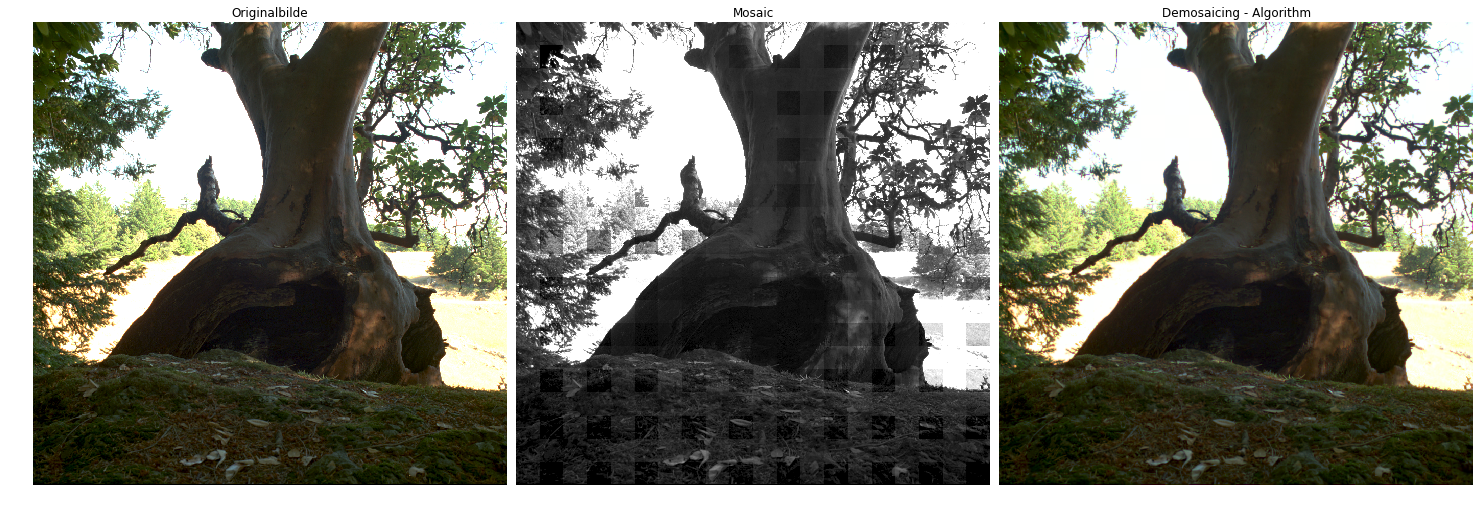
\includegraphics[width=1\columnwidth]{bilder/tree_mosaic.png} \label{Figur 3}
    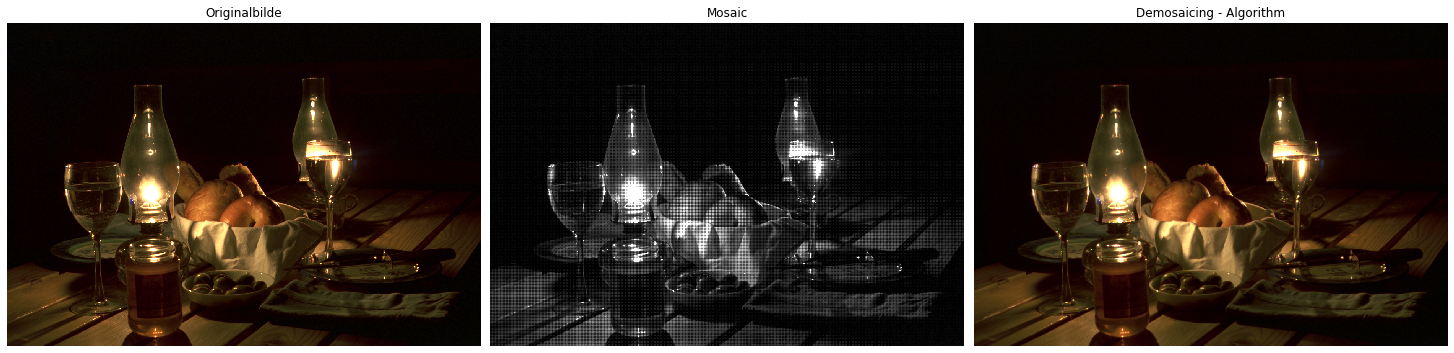
\includegraphics[width=1\columnwidth]{bilder/stillLife_mosaic.png}
    \caption{Demosaicing \label{Figur 4}}
\end{center}
\end{figure}
Resultatet av vår implementasjon vises i \ref{Figur 4}. Først presenteres originalbildet slik det blir lastet inn ved \texttt{imageio.imread}\footnote{\url{https://pypi.org/project/imageio/}}. Deretter vises gråtonemosaikken, før det ferdig interpolerte bildet. 